\section{Vorbereitung}

Die Vorbereitungsphase umfasst unter anderem die Umstellung der
Steuerungssoftware auf FreeRTOS und damit die vollständige Ablösung von
Micro-ROS. Der Datenaustausch wird intern über FreeRTOS-Queues realisiert,
während die Task-Synchronisation auf die leichtgewichtige
Direct-Task-Notification basiert. Zusätzlich wird die Methode zur Eingabe von
Sollgeschwindigkeiten über UART mit CRC-Überprüfung implementiert. Die
Aktivierung von Caches bildet den Abschluss dieser Vorbereitungen. Die Details
zu diesen Maßnahmen werden in den folgenden Abschnitten erläutert.

\subsection{Umstellung auf FreeRTOS}

\subsubsection{Empfang von Sollgeschwindigkeiten}

In der bisherigen Implementierung wurden Geschwindigkeitssollwerte vom
Micro-ROS-Agent über das ROS2-Framework an den Client auf den MCU übertragen. Um
die Abhängigkeit von Micro-ROS komplett zu beseitigen, muss die Übertragung nun
manuell entwickelt werden.

Es wird zunächst ein einfacher Struct \mintinline{cpp}|Vel2d| definiert, um die
Geschwindigkeitswerte zu aggregieren, die vom Benutzer an den MCU gesendet
werden.

\begin{code}
\begin{minted}{cpp}
struct Vel2d {
  double x;
  double y;
  double z;
};
\end{minted}
    \captionof{listing}{Definition der Struktur für die Sollgeschwindigkeit}
\end{code}

Darauf aufbauend wird eine weitere Struct \mintinline{cpp}|Vel2dFrame|
definiert, die als UART-Daten-Frame dient. Dieser enthält ein zusätzliches Feld
\mintinline{cpp}|crc| für die CRC-Überprüfung und eine Methode
\mintinline{cpp}|compare()|, die den nachträglich kalkulierten CRC-Wert als
Parameter entgegennimmt, um diesen mit dem vorhandenen zu vergleichen. Mit dem
Attribut \linebreak\mintinline{cpp}|__attribute__((packed))| wird verhindert,
dass zusätzliches Padding für die Speicherausrichtung dieses Typs eingefügt
wird.

\begin{code}
\begin{minted}{cpp}
struct Vel2dFrame {
  Vel2d vel;
  uint32_t crc;

  bool compare(uint32_t rhs) { return crc == rhs; }
} __attribute__((packed));

inline constexpr std::size_t VEL2D_FRAME_LEN = sizeof(Vel2dFrame);
\end{minted}
    \captionof{listing}{Definition der Data-Frame für die Sollgeschwindigkeit}
\end{code}

Für die Übertragung über UART kann die Funktion
\mintinline{cpp}|HAL_UARTEx_ReceiveToIdle_IT()| aus der STM32-HAL-Bibliothek
verwendet werden, um die serialisierten Bytes eines Data-Frames in den
vorallokierten Puffer zu empfangen.

Dies ist gepaart mit einer Interrupt-Callback
\mintinline{cpp}|HAL_UARTEx_RxEventCallback()|, die entweder ausgelöst wird,
wenn -- wie der Name der zugehörigen UART-Übertragungsfunktion bereits andeutet
-- die UART-Leitung feststellt, dass die Übertragung für eine bestimmte Zeit
(abhängig von der Baudrate) inaktiv war, oder wenn der Puffer einmal komplett
voll beschrieben wird~\cite{HAL_UARTEx_ReceiveToIdle_IT}. Der zweite Parameter
dieser Interrupt-Callback gibt die Größe der in den Puffer geschriebenen Daten
an \cite{HAL_UARTEx_RxEventCallback}.

Mit diesem Setup kann die Software auf der MCU nun Bytes direkt von einem
Linux-Host über UART empfangen. Die CRC-Prüfung und die Funktion zum Empfang bis
zum Idle-Zustand gewährleisten eine fehlertolerante Übertragung.

\begin{code}
\begin{minted}{cpp}
// preallocated buffer with the exact size of a data frame
static uint8_t uart_rx_buf[VEL2D_FRAME_LEN];
volatile static uint16_t rx_len;

void HAL_UARTEx_RxEventCallback(UART_HandleTypeDef* huart, uint16_t size) {
  if (huart->Instance != huart3.Instance) return;

  rx_len = size;
  static BaseType_t xHigherPriorityTaskWoken;
  configASSERT(task_handle != NULL);
  vTaskNotifyGiveFromISR(task_handle, &xHigherPriorityTaskWoken);
  portYIELD_FROM_ISR(xHigherPriorityTaskWoken);

  // reset reception from UART
  HAL_UARTEx_ReceiveToIdle_IT(&huart3, uart_rx_buf, sizeof(uart_rx_buf));
}

// setup reception from UART in task init
HAL_UARTEx_ReceiveToIdle_IT(&huart3, uart_rx_buf, sizeof(uart_rx_buf));
\end{minted}
    \captionof{listing}{Nutzung STM32-API für den Datenempfang über UART via
    Interrupt}
\end{code}

Um die empfangenen Bytes zu parsen, ohne dies aber während der Ausführung der
Interrupt-Callback zu tun, wird eine eigenständige FreeRTOS-Task erstellt.
Dieser Task wird von der Interrupt-Callback mittels
\mintinline{cpp}|vTaskNotifyGiveFromISR()|
signalisiert~\ref{sec:direct_task_notification} und die empfangenen Bytes werden
wiederum in ein Data-Frame deserialisiert, um die Geschwindigkeit und die CRC zu
extrahieren.

Demnach lässt sich zur Kontrolle eine CRC lokal aus den empfangenen
Geschwindigkeitswerten berechnen und mit der empfangenen vergleichen. Dabei
kommt die dedizierte CRC-Hardware zum Einsatz, die beispielsweise auf einem
STM32-F37x-Gerät die Berechnung um das 60-fache beschleunigt und dabei nur 1,6\%
der Taktzyklen im Vergleich zur Softwarelösung benötigt \cite[S. 9]{AN4187}.

\begin{code}
\begin{minted}{cpp}
  while (true) {
    ulTaskNotifyTake(pdTRUE, portMAX_DELAY);

    len = rx_len;  // access atomic by default on ARM
    if (len != VEL2D_FRAME_LEN) {
      ULOG_ERROR("parsing velocity failed: insufficient bytes received");
      continue;
    }

    auto frame = *reinterpret_cast<const Vel2dFrame*>(uart_rx_buf);
    auto* vel_data = reinterpret_cast<uint8_t*>(&frame.vel);
    if (!frame.compare(HAL_CRC_Calculate(
            &hcrc, reinterpret_cast<uint32_t*>(vel_data), sizeof(frame.vel)))) {
      ULOG_ERROR("crc mismatch!");
      ++crc_err;
      continue;
    }

    frame.vel.x *= 1000;  // m to mm
    frame.vel.y *= 1000;  // m to mm

    xQueueSend(freertos::vel_sp_queue, &frame.vel, NO_BLOCK);
  }
\end{minted}
    \captionof{listing}{FreeRTOS-Task Dauerschleife}
\end{code}

\subsubsection{Übertragung von Sollgeschwindigkeiten}

Um die vom Benutzer festzulegenden Geschwindigkeitssollwerten für den mobilen
Roboter zu übertragen, ist der MCU, auf dem die Steuerungssoftware
läuft, per UART mit einem Linux-Host verbunden. Auf dem Host wird das vorhandene
ROS2-Paket \mintinline{text}|teleop_twist_keyboard| weiter verwendet, um
Geschwindigkeitseingaben über die Tastatur zu realisieren. Um die Werten dann
über UART zu übertragen, wird ein kleiner ROS2-Node als Brücke erstellt.

Dabei empfängt der Node über das ROS2-Framework die Geschwindigkeitssollwerte
und überträgt sie zusammen mit der im Konstruktur kalkulierten CRC an die
UART-Schnittstelle, die auf Linux als abstrahierter serieller Port geöffnet ist.

\begin{code}
\begin{minted}{cpp}
class Vel2dBridge : public rclcpp::Node {
 public:
  Vel2dBridge() : Node{"vel2d_bridge"} {
    twist_sub_ = create_subscription<Twist>(
        "cmd_vel", 10, [this](Twist::UniquePtr twist) {
          auto frame =
              Vel2dFrame{{twist->linear.x, twist->linear.y, twist->angular.z}};

          if (!uart.send(frame.data())) {
            RCLCPP_ERROR(this->get_logger(), "write failed");
            return;
          }
          RCLCPP_INFO(this->get_logger(), "sending [%f, %f, %f], crc: %u",
                      frame.vel.x, frame.vel.y, frame.vel.z, frame.crc);
        });
  }

 private:
  rclcpp::Subscription<Twist>::SharedPtr twist_sub_;
  SerialPort<VEL2D_FRAME_LEN> uart =
      SerialPort<VEL2D_FRAME_LEN>(DEFAULT_PORT, B115200);
};
\end{minted}
    \captionof{listing}{ROS2-Node Implementierung für
    Geschwindigkeitsübertragung}
\end{code}

Die CRC-Berechnung auf dem Host erfolgt mithilfe einer C++-Bibliothek von Daniel
Bahr \cite{CRCpp}. Der Algorithmus \mintinline{cpp}|CRC::CRC_32_MPEG2()|
entspricht demjenigen, der von der CRC-Hardware des STM32-Boards verwendet wird.

\begin{code}
\begin{minted}{cpp}
Vel2dFrame::Vel2dFrame(Vel2d vel)
    : vel{std::move(vel)},
      crc{CRC::Calculate(&vel, sizeof(vel), CRC::CRC_32_MPEG2())} {}
\end{minted}
    \captionof{listing}{CRC-Berechnung im Konstruktur}
\end{code}

Mithilfe dieser Implementierungen werden die Übertragung von
Geschwindigkeitssollwerten vom Host und deren Empfang auf dem MCU ermöglicht.

\subsubsection{Steuerungskomponenten als FreeRTOS-Tasks}
\label{sec:freertos_tasks}

Ähnlich wie bei der Micro-ROS-Implementierung, wo alle logischen Komponenten als
Single-Threaded-Executor abstrahiert wurden, sind diese Komponenten in FreeRTOS
als eigenständige Tasks umgesetzt. Der Schwerpunkt liegt darauf, den
grundlegenden Datenaustausch ebenfalls über eine
Publisher-Subscriber-Architektur mit Queues zu realisieren. Dadurch entfällt die
Notwendigkeit, gemeinsame Daten mit Semaphoren oder Mutexen zu schützen, die in
FreeRTOS ohnehin nur als Queue-Objekte abstrahiert sind.

Zunächst wird eine eigenständige Task für die Abfrage und Übertragung der
Encoderwerte erstellt, die von der Hardware bzw. Hardwareabstraktion
bereitgestellt werden. Dadurch wird gewährleistet, dass alle anderen Tasks in
jeder Iteration auf konsistente Encoderwerte zugreifen können.

\begin{code}
\begin{minted}{cpp}
static void task_impl(void*) {
  constexpr TickType_t NO_BLOCK = 0;
  TickType_t xLastWakeTime = xTaskGetTickCount();
  const TickType_t xFrequency = pdMS_TO_TICKS(WHEEL_CTRL_PERIOD_MS.count());

  while (true) {
    auto enc_delta = FourWheelData(hal_encoder_delta_rad());

    xQueueSend(freertos::enc_delta_wheel_ctrl_queue, &enc_delta, NO_BLOCK);
    xQueueOverwrite(freertos::enc_delta_odom_queue, &enc_delta);

    vTaskDelayUntil(&xLastWakeTime, xFrequency);
  }
}
\end{minted}
    \captionof{listing}{FreeRTOS-Task für Encoderwertabfrage und -übertragung}
\end{code}


Die Empfänger-Task, welche mit \mintinline{cpp}|xQueueSend()| addressiert wird,
kann mit einer höhreren Frequenz laufen. Dabei arbeitet sie die Daten immer
schneller ab und wartet auf neue Daten. Im Gegensatz dazu ist
\mintinline{cpp}|xQueueOverwrite()| eine spezielle Funktion, die ausschließlich
für Queues mit einer maximalen Kapazität von einem Objekt vorgesehen ist. Sie
überschreibt das vorhandene Objekt in der Queue, falls es existiert. In diesem
Kontext ist dies jedoch irrelevant, da die zugehörige Empfänger-Task, der mit
der gleichen Frequenz wie die Encoderwert-Task läuft, die Daten synchron
verarbeitet. Dennoch dient die Überschreibbarkeit als zusätzliche
Sicherheitsmaßnahme für den Fall einer Verzögerung.

Darauf basierend kann die Kommunikation als Matrix wie folgt illustriert werden:

\begin{table}[h!]
\centering
\small
\setlength{\tabcolsep}{4pt} % Reduce column padding
\begin{tabular}{|c|c|c|c|}
\hline
    \diagbox{Sendertask}{Empfängertask} & \textbf{Odometrie} & \textbf{Drehzahlregelung} & \textbf{Posenregelung} \\ \hline
\textbf{Encoderwerte}               & $\rightarrow$             & $\rightarrow$       &               \\ \hline
\textbf{Geschwindigkeitssollwert}   &                           &                     & $\rightarrow$ \\ \hline
\textbf{Odometrie}                  & \cellcolor{gray!20}       &                     & $\rightarrow$ \\ \hline
\textbf{Drehzahlregelung}           &                           & \cellcolor{gray!20} & $\rightarrow$ \\ \hline
\end{tabular}
\caption{Kommunikationskanal-Matrix}
% \label{tab:kommunikationsmatrix}
\end{table}

Die Kanäle werden dementsprechend durch Queue-Objekte repräsentiert.

\begin{code}
\begin{minted}{cpp}
extern QueueHandle_t enc_delta_odom_queue;
extern QueueHandle_t enc_delta_wheel_ctrl_queue;
extern QueueHandle_t vel_sp_queue;
extern QueueHandle_t odom_queue;
extern QueueHandle_t vel_wheel_queue;
\end{minted}
    \captionof{listing}{Deklaration der Queue-Objekte in der Header-Datei}
\end{code}

Die grundlegende Implementierung der jeweiligen Steuerungstasks bleibt
größententeils von der Micro-ROS-Struktur erhalten. Die Initialisierung der
jeweiligen Steuerungstasks erfolgt in \mintinline{cpp}|freertos::init()|:

\begin{code}
\begin{minted}{cpp}
void init() {
  hal_init();
  queues_init();
  task_hal_fetch_init();
  task_vel_recv_init();
  task_pose_ctrl_init();
  task_wheel_ctrl_init();
  task_odom_init();
}
\end{minted}
    \captionof{listing}{Initialisierung von FreeRTOS-Tasks}
\end{code}

Eine üblicher Ansatz in einem FreeRTOS-System, um unter anderem sowohl den
Speicherverbrauch zu optimieren als auch die Determiniertheit zu verbessern,
besteht darin, die Erstellung der FreeRTOS-Objekte statisch durchzuführen
\cite{freertos_memory_management}.

Um diese zu realisieren, wird im Makefile ein Makro
\mintinline{text}|-DFREERTOS_STATIC_INIT| definiert, womit zur Übersetzungszeit
entschieden wird, ob die Objekte dynamisch oder statisch mit vorallokierten
Speicherorten zugewiesen werden sollen.

Für eine Task, deren Speicher dynamisch allokiert wird, ist die Initialisierung
wie folgt:

\begin{code}
\begin{minted}{cpp}
xTaskCreate(task_impl, "hal_fetch", STACK_SIZE, NULL, osPriorityNormal,
            &task_handle);
\end{minted}
    \captionof{listing}{Dynamische Allokation eines FreeRTOS-Tasks}
\end{code}

Wenn eine Task mit statischem Speicher erzeugt werden soll, muss der Nutzer
manuell sowohl einen Speicherpuffer für den Task-Stack, als auch für die
Task-Struktur selbst allokieren und an die API übergeben.

\begin{code}
\begin{minted}{cpp}
static StackType_t taskStack[STACK_SIZE];
static StaticTask_t taskBuffer;
task_handle = xTaskCreateStatic(
                    task_impl, "hal_fetch", STACK_SIZE, NULL, osPriorityNormal,
                    taskStack, &taskBuffer);
\end{minted}
    \captionof{listing}{Statische Allokation eines FreeRTOS-Tasks}
\end{code}

Analog dazu muss der Nutzer für eine statische Erzeugung einer Queue ebanfalls
jeweils einen Speicherpuffer mit der maximalen Kapazität für die Queue und die
Queue-Struktur selbst deklarieren:

\begin{code}
\begin{minted}{cpp}
 constexpr size_t QUEUE_SIZE = 10;
 static FourWheelData buf[QUEUE_SIZE];
 static StaticQueue_t static_queue;
 return xQueueCreateStatic(QUEUE_SIZE, sizeof(*buf),
                           reinterpret_cast<uint8_t*>(buf), &static_queue);
\end{minted}
    \captionof{listing}{Statische Allokation einer FreeRTOS-Queue}
\end{code}

Damit schließt der Abschnitt zur Umstellung auf FreeRTOS. Der Code für die
MCU-Software sowie für den ROS2-Node befindet sich im
Repository~\cite{mecarover_freertos_profiling} unter dem Branch
\mintinline{text}|freertos-profiling|.

\subsection{Aktivierung von Instruktionscache}

Zum Aktivieren des Instruktionscaches muss die Funktion
\mintinline{cpp}|SCB_EnableICache()| aufgerufen werden. Da der Instruktionscache
ausschließlich schreibgeschützte Befehle zwischenspeichert, ist keine
Synchronisation mit modifizierbaren Daten erforderlich.

\subsection{Aktivierung von Datencache}

Obwohl der Datencache ebenfalls durch den einfachen Funktionsaufruf
\mintinline{cpp}|SCB_EnableDCache()| aktiviert werden kann, stellt dies jedoch
noch nicht den abschließenden Schritt dar.

Die Transportfunktionen für Micro-ROS nutzen die Ethernet-Schnittstelle, deren
Funktionalität durch die Integration des LwIP-Stacks, der intern DMA verwendet,
erweitert wird. Um sicherzustellen, dass die Daten korrekt verarbeitet werden,
müssen sowohl der Heap für LwIP als auch die Speicherbereiche für die
Ethernet-RX- und TX-Deskriptoren mittels \ac{MPU} so konfiguriert werden, dass
sie nicht gecacht werden \cite{STM32H7_LwIP_Examples}.

\begin{figure}[H]
    \centering
    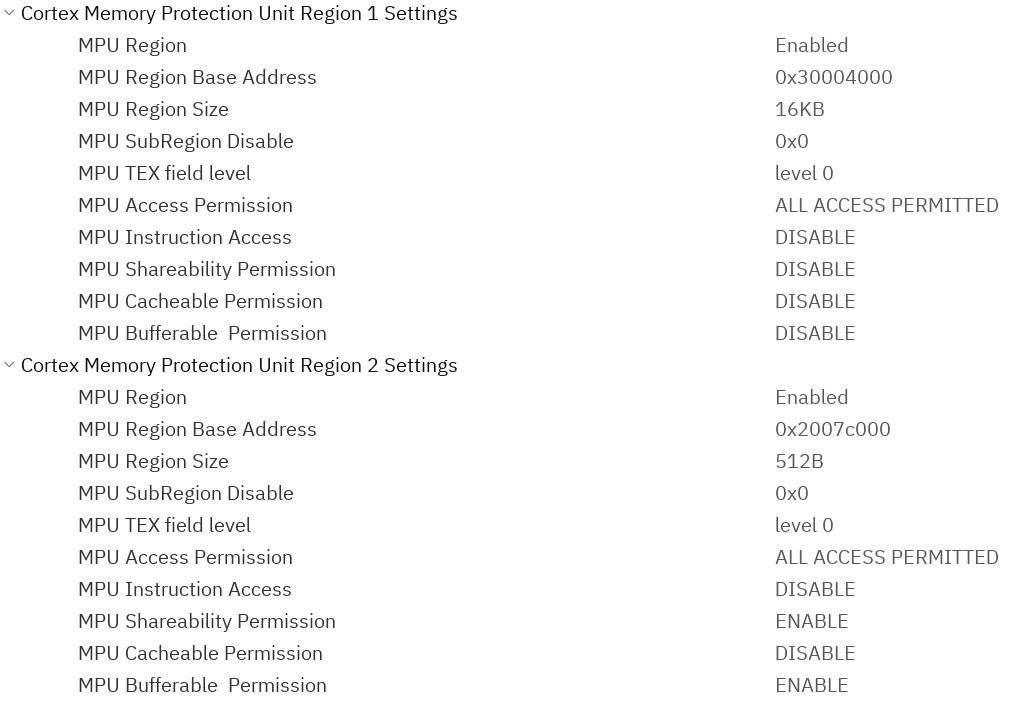
\includegraphics[width=1\textwidth]{assets/mpu_conf_cubemx}
    \caption{MPU-Konfiguration aus STM32CubeMX}
\end{figure}

Hierbei sind die Anfangsadressen sowie die Größe der RX- und TX-Deskriptoren
und des LwIP-Heaps aus CubeMX-Standardkonfigurationen entnommen.

Obwohl die MPU korrekt konfiguriert wurde, tritt dennoch ein Fehler auf, sobald
die Verbindung zum Micro-ROS-Client hergestellt wird. Der Fehler
(\ref{fig:micro_ros_err}), der in den Debugausgaben des Micro-ROS-Agents
sichtbar ist, deutet darauf hin, dass bei der Übertragung von Daten über UDP
weiterhin Probleme auftreten. Insbesondere scheint das
\mintinline{text}|client_key| bzw. die assoziierten Daten immer nicht ordentlich
gecacht zu werden.

\begin{figure}[H]
    \centering
    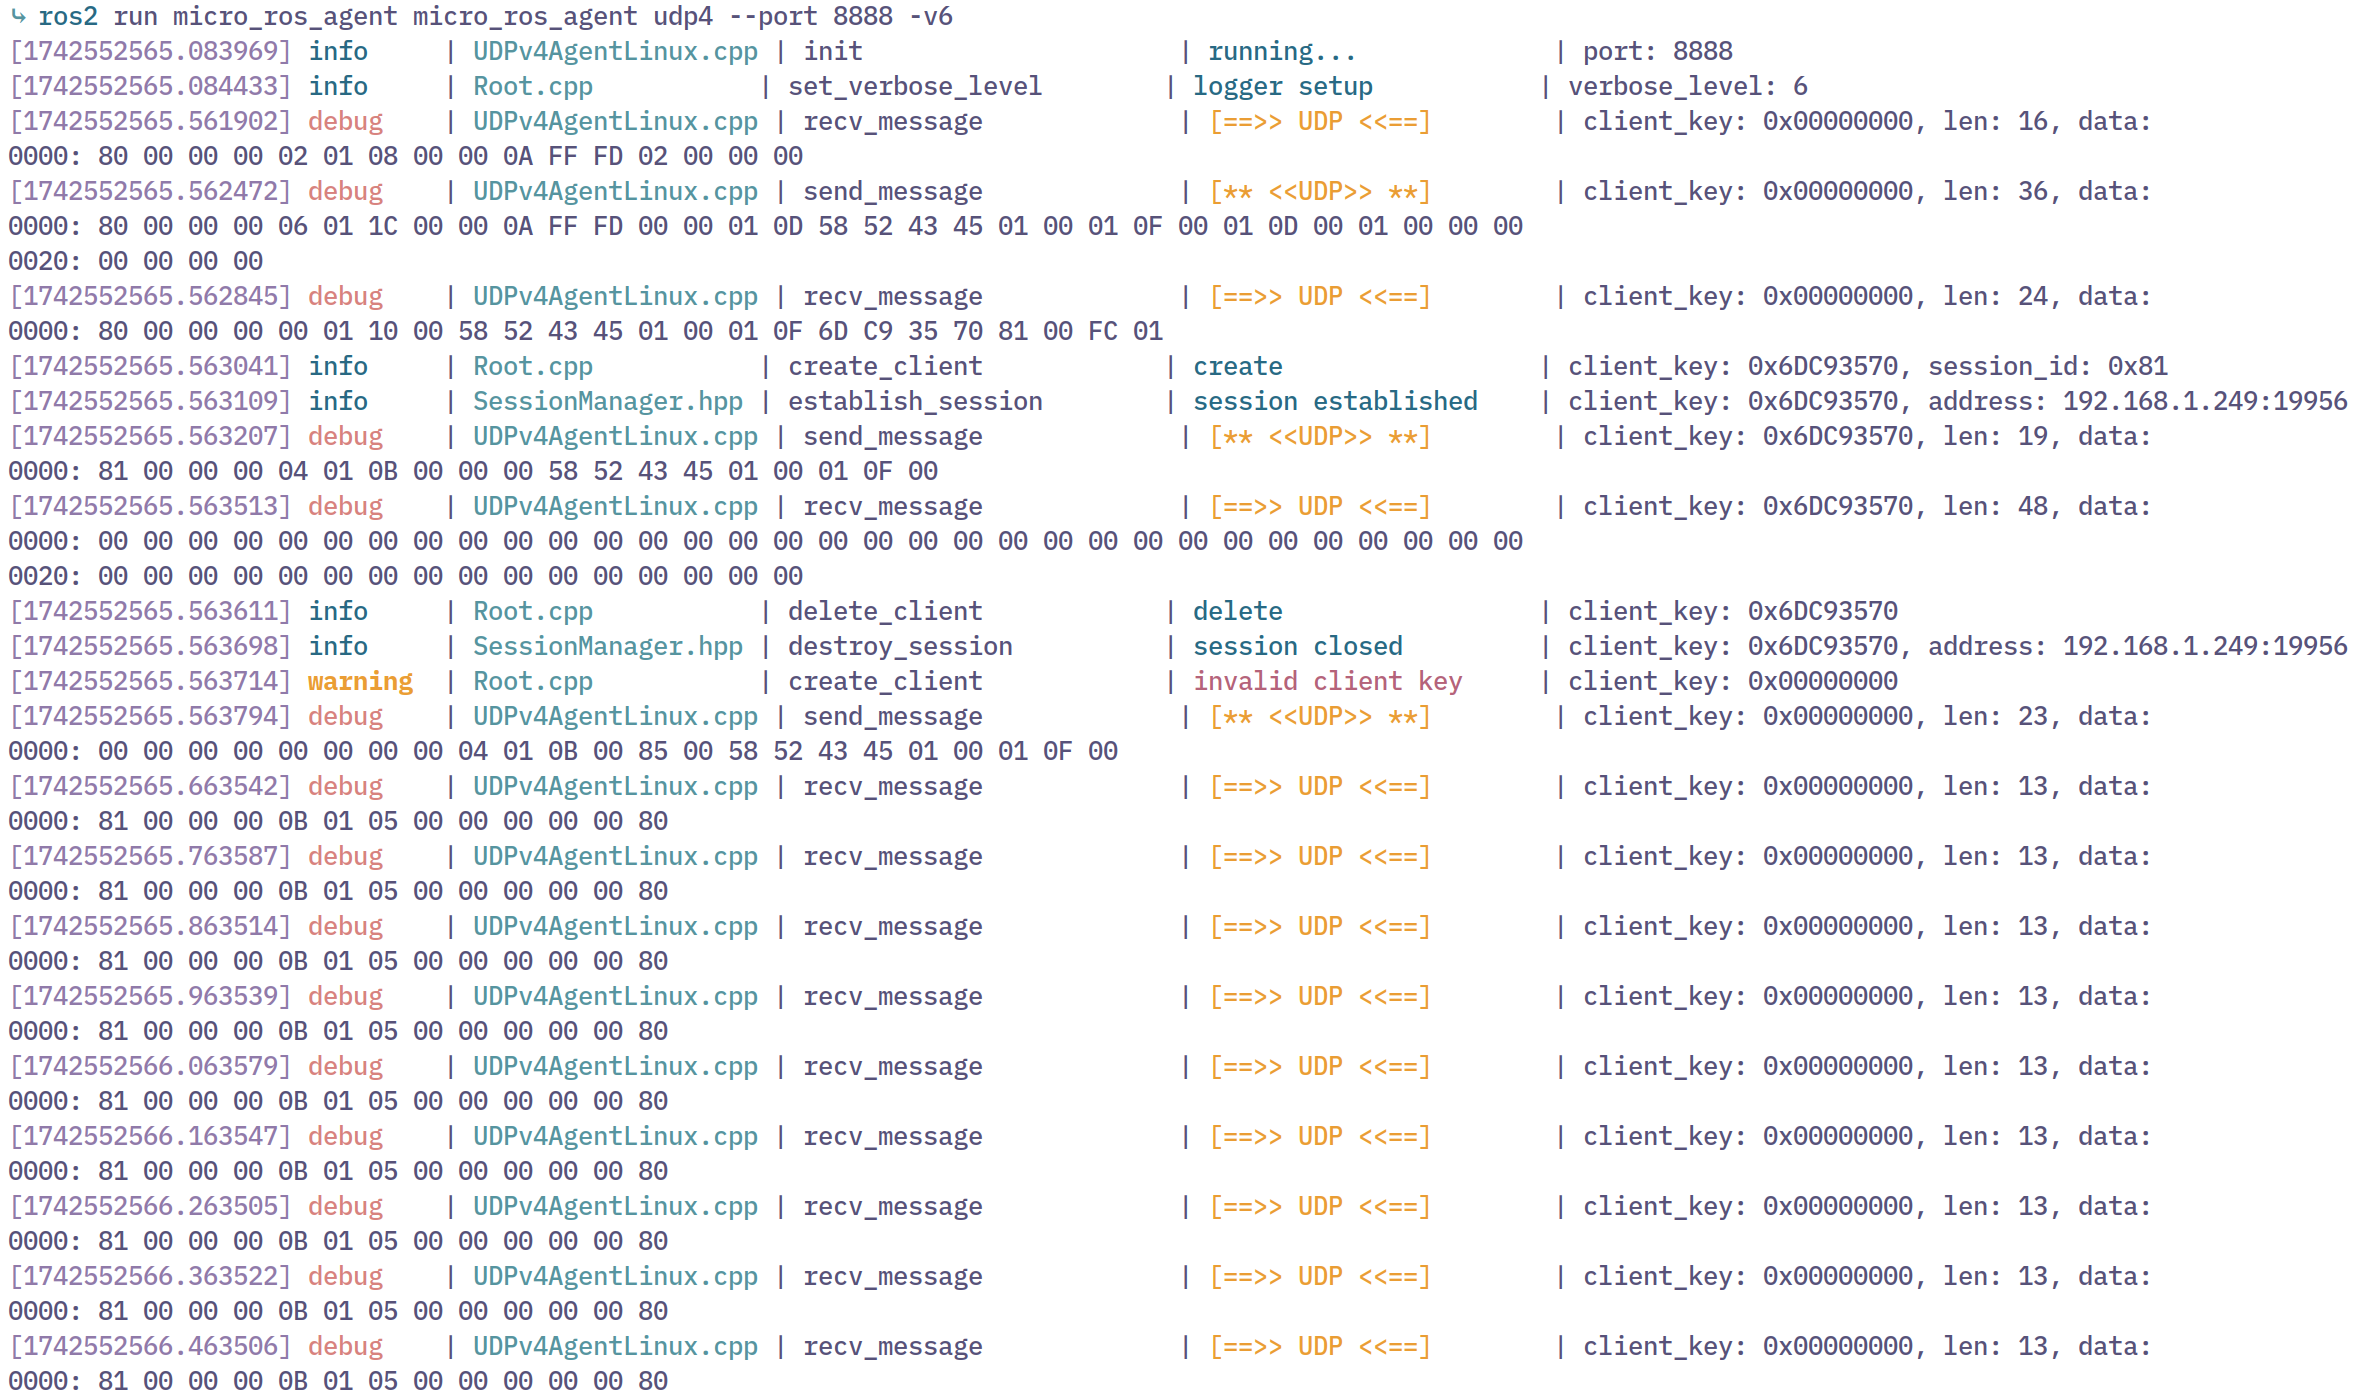
\includegraphics[width=1\textwidth]{assets/micro_ros_agent_err}
    \caption{Micro-ROS-Agent Fehlermeldung mit Debugausgaben}
    \label{fig:micro_ros_err}
\end{figure}

Bei der Recherche zu diesem Problem wurde ein Issue auf GitHub identifiziert,
welches genau das selbe Verhalten beschrieb. In diesem Kontext wurde dann der
Autor um eine Lösung gebeten, die daraufhin bereitgestellt wurde und sich als
effektiv erwies, um das Problem zu beheben \cite{microROS_STM32CubeMX_Issue139}.

\begin{code}
\begin{minted}{diff}
@@ -54,6 +54,10 @@
 /* USER CODE BEGIN 1 */
 /* address has to be aligned to 32 bytes */
+#define ALIGN_ADDR(addr) ((uintptr_t)(addr) & ~0x1F)
+#define ALIGN_SIZE(addr, size) ((size) + ((uintptr_t)(addr) & 0x1f))
+#define FLUSH_CACHE_BY_ADDR(addr, size) \
+  SCB_CleanDCache_by_Addr((uint32_t *)ALIGN_ADDR(addr), ALIGN_SIZE(addr, size))
 /* USER CODE END 1 */

 /* Private variables ---------------------------------------------------------*/
@@ -404,6 +408,8 @@
     Txbuffer[i].buffer = q->payload;
     Txbuffer[i].len = q->len;

+    FLUSH_CACHE_BY_ADDR(Txbuffer[i].buffer, Txbuffer[i].len);
+
     if(i>0)
     {
       Txbuffer[i-1].next = &Txbuffer[i];
\end{minted}
    \captionof{listing}{Modifizierung des ST-Treiber-Quellcode in Diffansicht
    \cite{microROS_STM32CubeMX_Issue139_code}}
    \label{code:cache_clean}
\end{code}

Die Lösung ist simple in Bezug auf den Codeumfang: Für jede Übertragung muss nur
der Cache für jeden Paketpuffer in \mintinline{cpp}|low_level_output()| mittels
den Funktionsaufruf \mintinline{cpp}|SCB_CleanDCache_by_Addr()| geleert werden
(\ref{sec:cache_clean}), so dass Änderungen von Daten tatsächlich in den
Speicher geschrieben und folglich auch beim DMA-Controller korrekt
widergespiegelt werden. Diese Lösung ist ebenfalls in einem Beitrag aus dem Jahr
2018 im ST-Forum dokumentiert \cite{ST_Forum_Post_2018}.

Da die Größe der Cachelines auf allen Cortex-M7-Prozessoren 32 Byte
beträgt~\cite[S. 4]{an4839} und bei jedem Caching die gesamte Cacheline gefüllt
wird, muss die übergebene Speicheradresse als Parameter durch eine bitweise
AND-Operation mit \mintinline{text}|~0x1F| auf eine 32-Byte-Grenze ausgerichtet
werden~\cite{CMSIS_Core_CacheFunctions}. Nach der Anpassung der Adresse für die
32-Byte-Ausrichtung muss die Größe dementsprechend wieder ergänzt werden, um die
ausgegrenzten Bytes nach der Ausrichtung wieder zu berücksichtigen.

Hierbei ist zu beachten, dass ein Teil der Modifizierung direkt im generierten
ST-Treiber-Quellcode vorgenommen wird, der bei Neugenerierung überschrieben
wird. In der Funktion \mintinline{cpp}|low_level_output()| ist kein durch ST
bereitgestellter User-Code-Guard vorhanden, und ein manuell hinzugefügter
User-Code-Guard wird ebenfalls überschrieben. Um dieses Problem zu umgehen,
wurde eine Patch-Datei erstellt, die nach jeder Neugenerierung der
entsprechenden Datei \mintinline{text}|LWIP/Target/ethernetif.c| angewendet
werden muss.
